\documentclass[11pt]{article}

\usepackage{fullpage,graphicx,latexsym,picinpar,amsbsy,amsmath,amsfonts}



\setlength{\evensidemargin}{0.1in}
\setlength{\oddsidemargin}{0.1in}
\setlength{\textwidth}{6.6in}
\setlength{\topmargin}{0.0in}
\setlength{\textheight}{8.7in}
\setlength{\headheight}{0in}
\setlength{\headsep}{0in}
\setlength{\topsep}{0in}
\setlength{\itemsep}{0in}
\renewcommand{\baselinestretch}{1.1}
\parskip=0.080in

\newcommand{\parend}[1]{{\left( #1  \right) }}
\newcommand{\spparend}[1]{{\left(\, #1  \,\right) }}
\newcommand{\angled}[1]{{\left\langle #1  \right\rangle }}
\newcommand{\brackd}[1]{{\left[ #1  \right] }}
\newcommand{\spbrackd}[1]{{\left[\, #1  \,\right] }}
\newcommand{\braced}[1]{{\left\{ #1  \right\} }}
\newcommand{\leftbraced}[1]{{\left\{ #1  \right. }}
\newcommand{\floor}[1]{{\left\lfloor #1\right\rfloor}}
\newcommand{\ceiling}[1]{{\left\lceil #1\right\rceil}}
\newcommand{\barred}[1]{{\left|#1\right|}}
\newcommand{\doublebarred}[1]{{\left|\left|#1\right|\right|}}
\newcommand{\spaced}[1]{{\, #1\, }}
\newcommand{\suchthat}{{\spaced{|}}}
\newcommand{\numof}{{\sharp}}

\newcommand{\half}{{\textstyle\frac{1}{2}}}
\newcommand{\elevenhalves}{{\textstyle\frac{11}{2}}}
\newcommand{\onethird}{{\textstyle\frac{1}{3}}}
\newcommand{\sixteenthirds}{{\textstyle\frac{16}{3}}}
\newcommand{\twentytwothirds}{{\textstyle\frac{22}{3}}}
\newcommand{\onefifth}{{\textstyle\frac{1}{5}}}
\newcommand{\threefifths}{{\textstyle\frac{3}{5}}}
\newcommand{\sixfifths}{{\textstyle\frac{6}{5}}}
\newcommand{\eightfifths}{{\textstyle\frac{8}{5}}}
\newcommand{\sixteenfifths}{{\textstyle\frac{16}{5}}}
\newcommand{\eightteenfifths}{{\textstyle\frac{18}{5}}}
\newcommand{\threetenths}{{\textstyle\frac{3}{10}}}
\newcommand{\twentysixfifteenths}{{\textstyle\frac{26}{15}}}
\newcommand{\fisefiftieths}{{\textstyle\frac{57}{50}}}
\newcommand{\ftwotfifths}{{\textstyle\frac{42}{25}}}
\newcommand{\fotwontwfifths}{{\textstyle\frac{42}{125}}}
\newcommand{\eithontwfifths}{{\textstyle\frac{83}{125}}}

\newcommand{\veps}{{\varepsilon}}
\newcommand{\Sigmastar}{{\Sigma^\ast}}

\newcounter{exnum}[section]
\newenvironment{problem}{{\vskip 0.1in
   \noindent \bf Problem\addtocounter{exnum}{1}~\arabic{exnum}.}}{\vskip 0.1in}

\newtheorem{theorem}{Theorem}
\newtheorem{definition}{Definition}
\newtheorem{corollary}{Corollary}
\newtheorem{lemma}{Lemma}
\newtheorem{fact}{Fact}
\newtheorem{claim}{Claim}

\newenvironment{proof}{{\it Proof:\/}}{$\Box$\vskip 0.1in}

\newcommand{\emparagraph}[1]{{\smallskip\noindent{\em #1\/}}}

\newcommand{\assign}{{\,\gets\,}}

%%%%%%%%%%%%%%%%%%%%%%%%%%%%%%%%%%%%%%%%%%%%%%%%%%%%%%%%%%%%%%%%%%%%%%%%%%%%%%%%%%%
%%%%%%%%%%%  LETTERS 
%%%%%%%%%%%%%%%%%%%%%%%%%%%%%%%%%%%%%%%%%%%%%%%%%%%%%%%%%%%%%%%%%%%%%%%%%%%%%%%%%%%

\newcommand{\barx}{{\bar x}}
\newcommand{\bary}{{\bar y}}
\newcommand{\barz}{{\bar z}}
\newcommand{\bart}{{\bar t}}

\newcommand{\bfP}{{\bf{P}}}

%%%%%%%%%%%%%%%%%%%%%%%%%%%%%%%%%%%%%%%%%%%%%%%%%%%%%%%%%%%%%%%%%%%%%%%%%%%%%%%%%%%
%%%%%%%%%%%%%%%%%%%%%%%%%%%%%%%%%%%%%%%%%%%%%%%%%%%%%%%%%%%%%%%%%%%%%%%%%%%%%%%%%%%
                                                                                  
\newcommand{\threehalfs}{\mbox{$\frac{3}{2}$}}   
\newcommand{\domino}[2]{\left[\frac{#1}{#2}\right]}  

%%%%%%%%%%%% complexity classes

\newcommand{\PP}{\mathbb{P}}
\newcommand{\NP}{\mathbb{NP}}
\newcommand{\PSPACE}{\mathbb{PSPACE}}
\newcommand{\coNP}{\textrm{co}\mathbb{NP}}
\newcommand{\DLOG}{\mathbb{L}}
\newcommand{\NLOG}{\mathbb{NL}}
\newcommand{\NL}{\mathbb{NL}}

%%%%%%%%%%% decision problems

\newcommand{\PCP}{\sc{PCP}}
\newcommand{\Path}{\sc{Path}}
\newcommand{\GenGeo}{\sc{Generalized Geography}}

\newcommand{\malytm}{{\mbox{\tiny TM}}}
\newcommand{\malycfg}{{\mbox{\tiny CFG}}}
\newcommand{\Atm}{\mbox{\rm A}_\malytm}
\newcommand{\complAtm}{{\overline{\mbox{\rm A}}}_\malytm}
\newcommand{\AllCFG}{{\mbox{\sc All}}_\malycfg}
\newcommand{\complAllCFG}{{\overline{\mbox{\sc All}}}_\malycfg}
\newcommand{\complL}{{\bar L}}
\newcommand{\TQBF}{\mbox{\sc TQBF}}
\newcommand{\SAT}{\mbox{\sc SAT}}

%%%%%%%%%%%%%%%%%%%%%%%%%%%%%%%%%%%%%%%%%%%%%%%%%%%%%%%%%%%%%%%%%%%%%%%%%%%%%%%%%%%
%%%%%%%%%%%%%%% for homeworks
%%%%%%%%%%%%%%%%%%%%%%%%%%%%%%%%%%%%%%%%%%%%%%%%%%%%%%%%%%%%%%%%%%%%%%%%%%%%%%%%%%%

\newcommand{\student}[2]{%
{\noindent\Large{ \emph{#1} SID {#2} } \hfill} \vskip 0.1in}

\newcommand{\assignment}[1]{\medskip\centerline{\large\bf CS 111 ASSIGNMENT {#1}}}

\newcommand{\duedate}[1]{{\centerline{due {#1}\medskip}}}     

\newcounter{problemnumber}                                                                                 


\newcounter{solutionnumber}

\newenvironment{solution}{{\vskip 0.1in \noindent
             \bf Solution~\addtocounter{solutionnumber}{1}\arabic{solutionnumber}:}}
				{\ \newline\smallskip\lineacross\smallskip}

\newcommand{\lineacross}{\noindent\mbox{}\hrulefill\mbox{}}

\newcommand{\decproblem}[3]{%
\medskip
\noindent
\begin{list}{\hfill}{\setlength{\labelsep}{0in}
                       \setlength{\topsep}{0in}
                       \setlength{\partopsep}{0in}
                       \setlength{\leftmargin}{0in}
                       \setlength{\listparindent}{0in}
                       \setlength{\labelwidth}{0.5in}
                       \setlength{\itemindent}{0in}
                       \setlength{\itemsep}{0in}
                     }
\item{{{\sc{#1}}:}}
                \begin{list}{\hfill}{\setlength{\labelsep}{0.1in}
                       \setlength{\topsep}{0in}
                       \setlength{\partopsep}{0in}
                       \setlength{\leftmargin}{0.5in}
                       \setlength{\labelwidth}{0.5in}
                       \setlength{\listparindent}{0in}
                       \setlength{\itemindent}{0in}
                       \setlength{\itemsep}{0in}
                       }
                \item{{\em Instance:\ }}{#2}
                \item{{\em Query:\ }}{#3}
                \end{list}
\end{list}
\medskip
}

%%%%%%%%%%%%%%%%%%%%%%%%%%%%%%%%%%%%%%%%%%%%%%%%%%%%%%%%%%%%%%%%%%%%%%%%%%%%%%%%%%%
%%%%%%%%%%%%% for quizzes
%%%%%%%%%%%%%%%%%%%%%%%%%%%%%%%%%%%%%%%%%%%%%%%%%%%%%%%%%%%%%%%%%%%%%%%%%%%%%%%%%%%

\newcommand{\quizheader}{ {\large NAME: \hskip 3in SID:\hfill}
                                \newline\lineacross \medskip }

%\newcommand{\namespace}{ {\large NAME: \hskip 3in SID:\hfill}
%                               \newline\lineacross \medskip }

%%%%%%%%%%%%%%%%%%%%%%%%%%%%%%%%%%%%%%%%%%%%%%%%%%%%%%%%%%%%%%%%%%%%%%%%%%%%%%%%%%%
%%%%%%%%%%%%% for final
%%%%%%%%%%%%%%%%%%%%%%%%%%%%%%%%%%%%%%%%%%%%%%%%%%%%%%%%%%%%%%%%%%%%%%%%%%%%%%%%%%%

\newcommand{\namespace}{\noindent{\Large NAME: \hfill SID:\hskip 1.5in\ }\\\medskip\noindent\mbox{}\hrulefill\mbox{}}





\begin{document}
	
% v -- YOUR NAME and SID in the braces
\student{ Nathan Ha}{ 862377326}  
% v -- YOUR NAME and SID in the braces
% \student{ name 2 }{sid 2 } 
% v -- ASSIGNMENT NUMBER in the braces
\assignment{ 3 } 
% v-- DUE DATE in the braces
\duedate{February 5, 2023 }  

\medskip

%%%%%%%%%%%%%%%%%%%%%%%%%%%%%%%%%%%%%%%%%%%%%%%%%%%%%%%%%%%%%%%%%%%%%%%%%%

\lineacross

%%%%%%%%%%%%%%%%%%%%%%%%%%%%
% problem 1
\begin{problem} \\
	\noindent a) Consider the following linear homogeneous recurrence relation: $R_n = 4R_{n-1} - 3R_{n-2}$. It is known that: $R_0 = 1$, $R_2 = 5$. Find $R_3$.

	\vspace {0.1in}
	\noindent b) Determine the general solution of the recurrence  equation if its characteristic equation has the following roots:  1, -2, -2, 2, 7, 7.

	\vspace {0.1in}
	\noindent  c) Determine the general solution of the recurrence  equation $A_n = 256A_{n-4}$.

	\vspace {0.1in}
	\noindent  d) Find the general form of the particular solution of the recurrence $B_n = 3B_{n-2} - 2B_{n-3}$ + 2.

\end{problem}

%---------------------------
% solution 1
\begin{solution} \\
	$(a)$ 
		This linear recurrence has a characteristic equation of $x^2 - 4x + 3 = 0$. This can be factored into $(x-3)(x-1) = 0 \implies x = 1, 3$. From here, we can write the general solution: 
		\\ $R_n = \alpha_1(1)^n + \alpha_2(3)^n = \alpha_1 + \alpha_2(3)^n$. We can now plug in $R_0$ and $R_2$ to solve for $\alpha$. 
		\\ $R_0 = 1 = \alpha_1 + \alpha_2$. 
		\\ $R_2 = 5 = \alpha_1 + \alpha_2(3)^2$. 
		\\ We can subtract the two equations to get $4 = 8\alpha_2 \implies \alpha_2 = \frac{1}{2}$.
		\\ Plugging in $\alpha_2$ into the first equation, we get $\alpha_{1,2} = \frac{1}{2}$. This means that the closed form for the recurrence is $R_n = \frac{1}{2}(3)^n + \frac{1}{2}$. We can plug in 3 and get $R_3 = \frac{1}{2}(3)^3 + \frac{1}{2} = 14$. 

	\text{}\\
	$(b)$
		A general solution of a recurrence with these roots would look like: \\ \text{}\quad\quad $R_n = \alpha_1(1)^n + \alpha_2(-2)^n + \alpha_3n(-2)^n + \alpha_4(2)^n + \alpha_5(7)^n + \alpha_6n(7)^n$.

	\text{}\\
	$(c)$
		The characteristic equation of this recurrence $x^4 - 256 = 0 \implies (x-4)(x+4)(x^2+16)=0 \\\implies (x-4)(x+4)(x+4i)(x-4i)=0$. The roots are $-4, 4, -4i, 4i$. The general solution to this is $R_n = \alpha_1(-4)^n + \alpha_2(4)^n + \alpha_3(-4i)^n + \alpha_4(4i)^n$.

	\text{}\\
	$(d)$
		At first glance, the general form of the particular solution is $B_n'' = \beta$. To be sure, though, we have to find the general form of the homogenous equation. The characteristic equation of the homogenous part is $x^3 - 3x + 2 = 0$. Using the rational root theorem and synthetic divison, we can factor this into $(x-1)^2(x+2)=0$. This means that $x = -2, 1$ (multiplicity 2). This means that the general form of the homogeneous solution is $B_n' = \alpha_1 (-2)^n + \alpha_3 + \alpha_4n$. Going back to the particular solution, we can see that $B_n'' = \beta$ will not work because it is a solution to the homogenous form. By the same logic, we can see that $B_n'' = \beta n$ will not work either. This means that the general form of the particular solution is $B_n'' = \beta n^2$.

	\end{solution}

%%%%%%%%%%%%%%%%%%%%%%%%%%%%
% problem 2
\newpage
\begin{problem}
	Solve the following recurrence equations:

%
$a)$
\begin{eqnarray*}
        f_n &=& f_{n-1} + 4f_{n-2} + 2f_{n-3}\\
        f_0 &=& 0 \\
        f_1 &=& 1 \\
		f_2 &=& 4 
\end{eqnarray*}
%
Show your work (all steps: the characteristic polynomial and its roots, the general solution, 
using the initial conditions to compute the final solution.)


$b)$
\begin{eqnarray*}
        t_n &=& t_{n-1} + 2t_{n-2} + 2^n\\
        t_0 &=& 0 \\
        t_1 &=& 2
\end{eqnarray*}
%
Show your work (all steps: the associated homogeneous equation,
the characteristic polynomial and its
roots, the general solution of the homogeneous
equation, computing a particular solution,
the general solution of the non-homogeneous equation,
using the initial conditions to compute the final solution.)
%
\end{problem}

\newpage
%-----------------------------
% solution 2
\begin{solution} \\
	$(a)$ 
		The characteristic equation of this recurrence is $x^3 - x^2 -4x - 2 = 0$. Using the rational root theorem, we know that one root of this polynomial must be $\pm1$, or $\pm 2$. Pluggin in -1 yields a true statement, therefore we can factor out an $x+1$ from the characteristic equation. Using synthetic division, we get: $(x+1)(x^2 - 2x - 2) = 0$. Using the quadratic equation, we can simplify the second degree factor and get: $(x+1)(x - (1 - \sqrt{3}))(x-(1+ \sqrt{3})) = 0$. Now that we have the roots, we can find the general solution to the recurrence: $f_n = \alpha_1(-1)^n + \alpha_2(1 - \sqrt{3})^n + \alpha_3(1 + \sqrt{3})^n $. We can now plug in the base cases to solve for the constants: 
		\\ $f_0 = 0 = \alpha_1 + \alpha_2 + \alpha_3$ 
		\\ $ f_1 = 1 = -\alpha_1 + \alpha_2(1-\sqrt{3}) + \alpha_3(1+\sqrt{3}) $ 
		\\ $ f_2 = 4 = \alpha_1 + \alpha_2(1-\sqrt{3})^2 + \alpha_3(1+\sqrt{3})^2 $ 
		\\ To solve this system, we can use Gauss-Jordan elimination: \\
		$
			\begin{pmatrix}
			1 & 1 & 1 & 0 \\
			-1 & (1-\sqrt{3}) & (1+\sqrt{3}) & 1 \\
			1 & (1-\sqrt{3})^2 & (1+\sqrt{3})^2 & 4
			\end{pmatrix} 
			% \implies
			\xrightarrow[\text{}]{\text{rref}}
			\begin{pmatrix}
				1 & 0 & 0 & 2 \\
				0 & 1 & 0 & \frac{-6 - 5\sqrt{3}}{6} \\
				0 & 0 & 1 & \frac{-6 + 5\sqrt{3}}{6}
			\end{pmatrix} 
		$
		\\ This means that the solutions are: $\alpha_{1,2,3} = 2, \frac{-6 - 5\sqrt{3}}{6}, \frac{-6 + 5\sqrt{3}}{6} $. Thus, the solution of the recurrence is $f_n = 2(-1)^n + \frac{-6 - 5\sqrt{3}}{6}(1 - \sqrt{3})^n + \frac{-6 + 5\sqrt{3}}{6}(1 + \sqrt{3})^n $.
	\\\\\\
	$(b)$ To solve this recurrence, we need to first solve the homogeneous part and the nonhomogenous parts of the recurrence. The characteristic equation of the homogeneous part is $x^2 - x - 2 = 0 \implies x_{1,2} = -1, 2$. This gives us $t_n' = \alpha_1 (-1)^n + \alpha_2 (2)^n$.
	\\\\ For the nonhomogenous, we should recognize that the general form of the particular solution is $t_n'' = \beta 2^{n}$. The homogenous equation already has a $2^n$ multiplied by a constant, so we need to multiply the particular solution by n: $t_n'' = \beta n2^{n}$. To solve for $\beta$, we should plug in the particular solution into the recurrence: $\beta n2^n = \beta(n-1)2^{n-1} + 2\beta(n-2)2^{n-2} + 2^n$. Dividing this equation by $2^{n-2}$ yields: $4\beta n = 2\beta(n-1) + 2\beta (n-2) + 4$. Solving for $\beta$ gives $\beta = \frac{2}{3}$. This means that $t_n'' = \frac{2}{3}n 2^n$.
	\\\\ Combining the two, we find that the general form of the solution is $t_n = \alpha_1 (-1)^n + \alpha_2 (2^n) + \frac{2}{3}n2^n$. Plugging in the base cases gives:
	\\ $t_0 = 0 = \alpha_1 + \alpha_2$
	\\ $t_1 = 2 = -\alpha_1 + 2\alpha_2 + \frac{4}{3}$.
	\\ Add the two equations to get $2 = 3 \alpha_2 + \frac{4}{3} \implies \alpha_2 = \frac{2}{9}$.
	\\ Plugging $\alpha_2$ into the first equation gives us: $\alpha_1 = -\frac{2}{9}$. This means that the final solution is: $t_n = -\frac{2}{9}(-1)^n + \frac{2}{9}(2^n) + \frac{2}{3}n2^n$.

	\end{solution}

%%%%%%%%%%%%%%%%%%%%%%%%%%%
% problem 3
\newpage
\begin{problem}
	We want to tile an $n\times 1$ strip with $1\times 1$ tiles that are green (G), blue (B), and red (R), $2\times 1$ purple (P) and $2\times 1$ orange (O) tiles. Green, blue and purple tiles cannot be next to each other, and there should be no two purple or three blue or green tiles in a row (for ex., GGOBR is allowed, but GGGOBR, GROPP and PBOBR are not). Give a formula for the number of such tilings. Your solution must include a recurrence equation (with initial conditions!), and a full justification. You do not need to solve it. 
\end{problem}

%----------------------------
% solution 3
\begin{solution}
	\\   Just for reference, note that the following patterns are NOT allowed: GB, BG, GP, PG, BP, PB, PP, BBB, GGG. We now have to break up the tilings into its most basic components. Also, let's say that the number of tilings is $T_n$. 
	\\\\ First, we can look at the easiest cases: inserting an R will give a tile with $T_{n-1}$ possible tilings left. Similarly, inserting an O will give $T_{n-2}$ possible tilings. Since R and O have no restrictions on what they can be next to, we don't have to do anything else with them. 
	\\\\ Now let's look at the next simplest case: inserting a P. Since P cannot be next to a G,P, or B, it must be either next to a R or and O. This will leave you with $T_{n-3}$ and $T_{n-4}$ possible tilings respectively. 
	\\\\ Green and Blue are more complicated, but they both behave the same in terms of the restrictions placed on them. Let's say you insert a G. Since R and O have no restrictions, we can freely place them next to G. Placing an R leaves $T_{n-2}$ possible tilings left, and placing an O will leave $T_{n-3}$ left. If you place a G next to the G, in order to prevent 3 G's in a row, we have to place either a R or an O. Placing them will leave $T_{n-3}$ and $T_{n-4}$ remaining tilings respectively. 
	\\\\ Again, G and B behave exactly the same, so we can just multiply the tilings for the above paragraph by 2. Adding up all the possible tilings gives: \\ $T_n = 2(T_{n-2} + T_{n-3} + T_{n-3} + T_{n-4}) + T_{n-2} + T_{n-1} + T_{n-3} + T_{n-4} \\ =  3T_{n-4} + 5T_{n-3} + 3T_{n-2} + T_{n-1}$.
	\\\\ Since this recurrence is 4th degree, we need 4 base cases. We can say $T_0 = 1$ because there is only one way to tile 0 tiles. $T_1 = 3$ because there are three tiles that will fit in a 1x1 slot. $T_2 = 9$ because there are two 2x1 tiles plus seven ways to arrange 1x1 tiles (RG, RB, GG, BB, RR, GR, GB). Following similar logic, we can see that $T_3 = 23$. \footnote[1]{The possible combinations for this case are OG, GO, OB, BO, OR, RO, PR, RP, GGR, GRG, GRR, RGG, RGR, RRG, RRR, BBR, BRB, BRR, RBB, RBR, RRB, BRG, GRB.} Below is a tree representation of this recursion.
	\\\\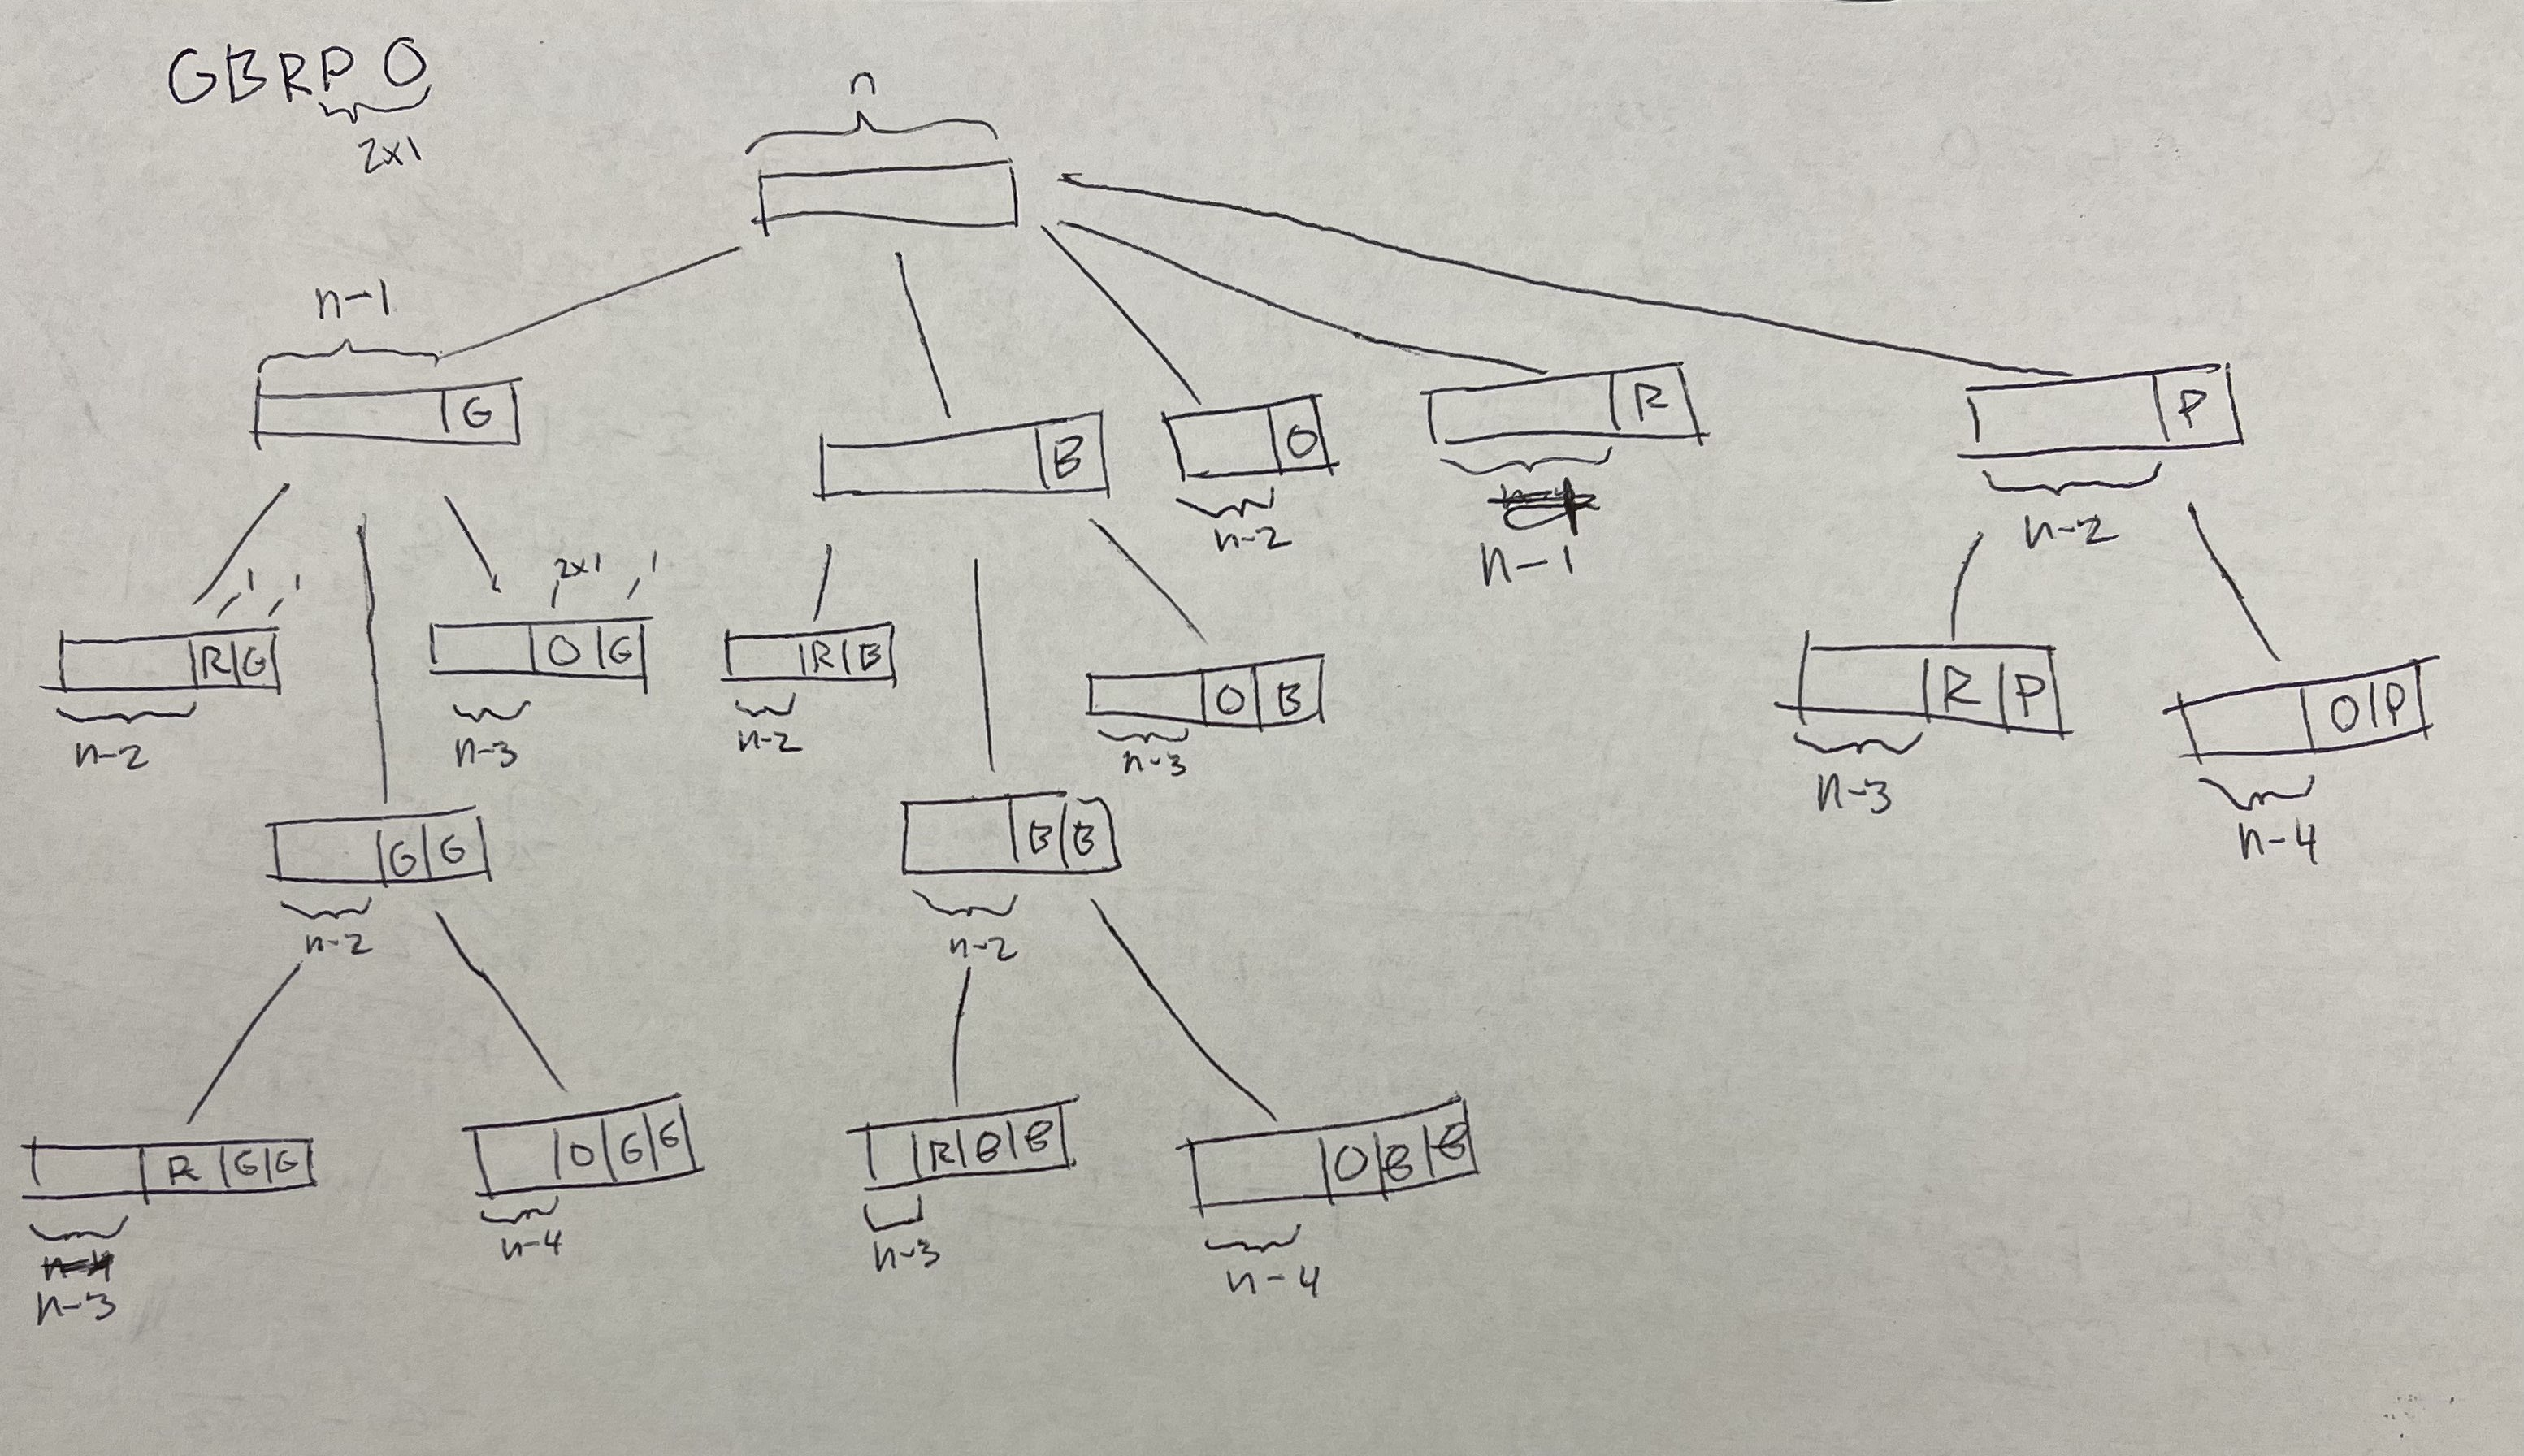
\includegraphics[scale=0.05]{q3tree.jpg}
\end{solution}

%%%%%%%%%%%%%%%%%%%%%%%%%%%%
\newpage
\vskip 0.1in

\paragraph{Academic integrity declaration.}
I did this homework on my own. I got a lot of help during office hours, though.


\end{document}

